\documentclass{ohm_project_description}

\projecttitle{Drone Swarm Obstacle Avoidance – Kollisionsfreie Navigation von Micro-Drohnen}
\projectauthor{Labor für mobile Robotik}
\projectdate{2026}

\begin{document}

\maketitle
\thispagestyle{fancy}

\vspace*{-2.5cm}
\begin{figure}[h!]
    \centering
    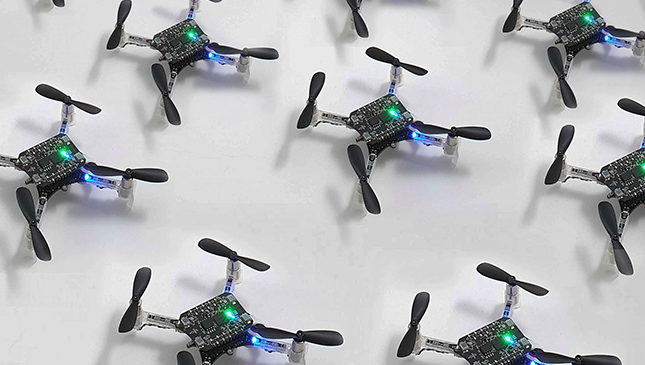
\includegraphics[height=4cm]{img/crazyflies.png}
\end{figure}

Die am AerodrOHM eingesetzten Micro-Drohnen (Crazyflies) verfügen über keine ausgeprägte Onboard-Sensorik zur Umgebungswahrnehmung. Um dennoch eine sichere Interaktion mit Personen im Flugraum zu ermöglichen, soll in diesem Projekt eine externe 3D-Kamera in der Nähe des Schwarms installiert werden. Das Ziel ist ein System, das Personen im gemeinsamen Flugraum zuverlässig erkennt und den Schwarm so steuert, dass die Drohnen automatisch ausweichen und Raum freigeben.

Im ersten Schritt soll die 3D-Kamera in eine ROS-basierte Systemarchitektur eingebunden werden. Ein zentraler Aspekt ist die Klassifikation der erfassten Objekte: Das System muss zuverlässig zwischen Personen und den Drohnen selbst unterscheiden können. Aufbauend auf der Personenerkennung soll ein reaktives Schwarmverhalten entwickelt werden, das eine sichere Koexistenz im gemeinsamen Raum gewährleistet. Die praktische Erprobung findet im Flugraum des AerodrOHM statt.

\section*{Arbeitspakete}
\begin{itemize}[leftmargin=0.5cm]
    \setlength\itemsep{.1em}
    \item Einbindung und Kalibrierung der externen 3D-Kamera
    \item Verarbeitung, Filterung und Transformation der Punktwolkendaten
    \item Entwicklung einer Klassifikation zur Unterscheidung von Personen und Drohnen
    \item Entwurf und Implementierung eines reaktiven Schwarmverhaltens mit Sicherheitszonen
    \item Test und Evaluation im Flugraum mit realen Personen
\end{itemize}

\section*{Voraussetzungen}
\begin{itemize}[leftmargin=0.5cm]
    \setlength\itemsep{.1em}
    \item Kenntnisse in Programmierung (Python und/oder C++)
    \item Idealerweise erste Erfahrungen mit ROS
    \item Interesse an Sensorintegration, Punktwolkenverarbeitung und Wahrnehmungsverfahren
\end{itemize}

\vspace{0.5cm}
Das Thema kann nach Abstimmung als \textbf{Projekt- oder Masterarbeit} bearbeitet werden.

\vfill
\textcolor{ohm_red}{\rule{\linewidth}{0.4mm}}
\textbf{\textcolor{ohm_red}{Labor für mobile Robotik}} \\
\begin{tabular}{@{}ll}
\textbf{Betreuer:} & Prof. Dr. Christian Pfitzner \\
\textbf{E-Mail:}   & \href{mailto:christian.pfitzner@th-nuernberg.de}{christian.pfitzner@th-nuernberg.de} \\
\end{tabular}

\end{document}
